% !Mode:: "TeX:UTF-8"
% -*-coding: utf-8 -*-

% Русский язык дополнительно настраивать не нужно.
% Убедитесь, что ваш редактор поддерживает UTF-8.
\documentclass{math-mech-sci}

% Название и авторы задаются при помощи специальных
% команд \deftitle и \defauthor. Специальные команды
% требуются для генерации корректной метаинформации в
% PDF-файле.

% Блоки в квадратных скобках опциональны, они предназначены
% для сносок на гранты, которыми поддержана работа.

\deftitle%
  [\thanks{В квадратных скобках опционально,
  кем и чем поддержана работа. Если никем и ничем,
  убираем вместе со скобками.}]%
  {Название статьи}

\defauthor%
  {Луцив Д.В.}%
  {СПбГУ, Санкт-Петербург}%
  {d.lutsiv@spbu.ru}
\defauthor%
  [\thanks{Или если был поддержан отдельный автор.}]%
  {Чижова А.С.}%
  {ООО «КНС-Групп», Санкт-Петербург}%
  {a.chizhova@yadro.com}

\begin{document}

\maketitle

\begin{abstract}
Данный документ представляет собой образец оформления материалов
Весенней научно-практической конференции
«Мат-мех. Наука 2024»,
и содержит базовый набор рекомендованных к использованию
макросов для форматирования текста.
\end{abstract}

\section{Введение}

Самый простой способ использовать образец --- просто заменить всё его
содержимое на своё, используя уже определённые в документе команды.

При этом:
\begin{itemize}
\item
  аккуратное использование данного шаблона позволит автору увидеть статью
  примерно с тем же форматированием, с которым она попадёт в сборник;
\item
  аккуратное использование данного шаблона облегчит труд верстальщика, а в итоге
  может даже ускорить издание сборника: в целом мат-меховские
  конференции подразумевают достаточно большое количество докладов,
  о чём свидетельствует Таблица~\ref{tab:math-science2011}.
\end{itemize}

\begin{table}[h]
\begin{center}
\begin{tabular}{|r|l|}
\hline
\thd{Показатель} & \thd{Значение} \tabularnewline
\hline
Всего секционных докладов & 130 \tabularnewline
\hline
Всего секций & 17 \tabularnewline
\hline
Страниц в сборнике & 480 \tabularnewline
\hline
\end{tabular}
\caption{Количественные показатели конференции
  СПИСОК-2011}\label{tab:math-science2011}
\end{center}
\end{table}

\section{Формат конференции (заголовок I уровня)}

Формат конференции подразумевает выступление с интересным и
содержательным докладом, по итогам доклада рекомендуются к публикации
в сборнике конференции материалы, в отношении которых справедливо:

\begin{itemize}
\item
  текст содержит:
  \begin{enumerate}
  \item
    аннотацию;
  \item
    введение;
  \item
    один или несколько разделов;
  \item
    заключение;
  \item
    список литературы;
  \end{enumerate}
\item
  предполагаемый объём текста, включая список литературы, от 4 до 7 страниц;
  если это требование нарушено, то решение о включении текста в
  сборник принимает программный комитет, опираясь, в основном, на
  мнение руководителя секции, на которой прозвучал доклад;
\item
  основной язык конференции русский, однако члены программного
  комитета могут приглашать иностранных докладчиков, тексты докладов
  которых могут публиковаться по-английски; публикации на прочих языках
  отдельно согласуются с программным комитетом.
\end{itemize}

\section{Форматирование тезисов (заголовок I уровня)}

\subsection{Основной текст (заголовок II уровня)}

Основной текст отформатирован следующим образом:

\begin{enumerate}
\item
  шрифт, метрически совместимый с Times\footnote{Для \ifxetex \XeLaTeX \else Xe\LaTeX \fi мы используем набор из Tempora, \textsf{Liberation Sans} и \texttt{Iosevka Extended}, которые метрически эквивалентны Times, Arial и Courier соответственно. Для PDF\LaTeX --- шрифты CM.  Чистовая вёрстка
  выполняется при помощи \ifxetex \XeLaTeX \else Xe\LaTeX \fi, будьте к этому готовы!}, кегль 10
\item
  первая и последующие страницы:

  \begin{enumerate}
  \item
    все поля, кроме верхнего, по 17 мм;
  \item
    верхнее поле 23 мм;
  \end{enumerate}
\item
  аннотация имеет дополнительные отступы по 10 мм слева и справа.
\end{enumerate}

\subsection{Формулы (заголовок II уровня)}

Включенные в текст формулы оформляются при помощи одиночных знаков доллара, например $e^{\pi i} + 1 = 0$.
Включенные формулы, содержащие "Большие" операторы начинаются с команды \verb"{\displaystyle ...}", например ${\displaystyle\int f(x)dx}$. Формулы, содержащие дроби, не следует делать включенными.

Выключенные дроби могут быть пронумерованы:

\begin{equation}
	\label{eq:exp1}
	\int u(x)v'(x)dx=u(x)v(x)-\int u'(x)v(x)dx,
\end{equation}

либо нет:

\begin{equation*}
	\int f(\varphi(x))\varphi'(x)dx=F(\varphi(x))+C.
\end{equation*}

Многострочные формулы:

\begin{equation}\label{eq:exp2}
\begin{array}{r@{}l}
	%N_{x,sk} &{}= k_{sk}\left(\frac{t_{sk}}{b_{sk}}\right)^{2}\bar{Et}\\
	%N_{x,st} &{}= k_{st}\left(\frac{t_{st}}{b_{st}}\right)^{2}\bar{Et}\\
	\sum^{k}_{s=1}(b_s-a_s)b^{2(\alpha-2)}_s  &= \\
	=c_s\sum^{k}_{s=1}\displaystyle\frac{1}{(4s+1)(4s-1)}\left(\displaystyle\frac{1}{4s-1}\right)^{2(\alpha-2)}
	&\geqslant c’_s\sum^{k}_{s=1}\displaystyle\frac{1}{s^{2\alpha-2}}.
\end{array}
\end{equation}

Последовательно следующие одна за другой формулы:
\begin{align}
	N_{x,sk} &= k_{sk}\left(\frac{t_{sk}}{b_{sk}}\right)^{2}\bar{Et}\\
	N_{x,st} &= k_{st}\left(\frac{t_{st}}{b_{st}}\right)^{2}\bar{Et}
\end{align}

При верстке выключенных формул не допускайте переполнения строки! Пример ссылки на формулу: \eqref{eq:exp1}.

\subsection{Определения, теоремы, доказательства, следствия (заголовок II уровня)}

Определения, теоремы, леммы, и т.п. нумеруются вручную, нумерация для них сквозная внутри тезисов. Оформление согласно приведенным ниже образцам.

\textbf{Определение 1.} Функция непрерывна в точке, если её колебание в данной точке равно нулю.

\textbf{Теорема 1.} (о свойстве Дарбу) Пусть дана непрерывная вещественнозначная функция на отрезке 
$f:[a,b]\subset \mathbb {R} \to \mathbb {R} ,\;f\in C^{0}{\bigl (}[a,b]{\bigr )}$. Тогда существуют
$ c,d\in \mathbb {R}$ такие, что

\begin{equation*}
	f{\bigl (}[a,b]{\bigr )}=[c,d].
\end{equation*}

\emph{\textbf{Доказательство.}} ....
	
	
\subsection{Цитаты, врезки изображений (заголовок II уровня)}

Ниже процитирован отрывок из Метафизики Аристотеля. Отметим, что
данная цитата несёт некоторую смысловую нагрузку и в контексте данного
документа, показывая, что цитаты следует выделять курсивом.

\emph{\ldots{} В самом деле, определенное умение читать и писать
  принадлежит к тому, что находится в подлежащем, но ни о каком
  подлежащем не говорится как об определенном умении читать и
  писать)\ldots}

\begin{figure}[h]
\begin{center}
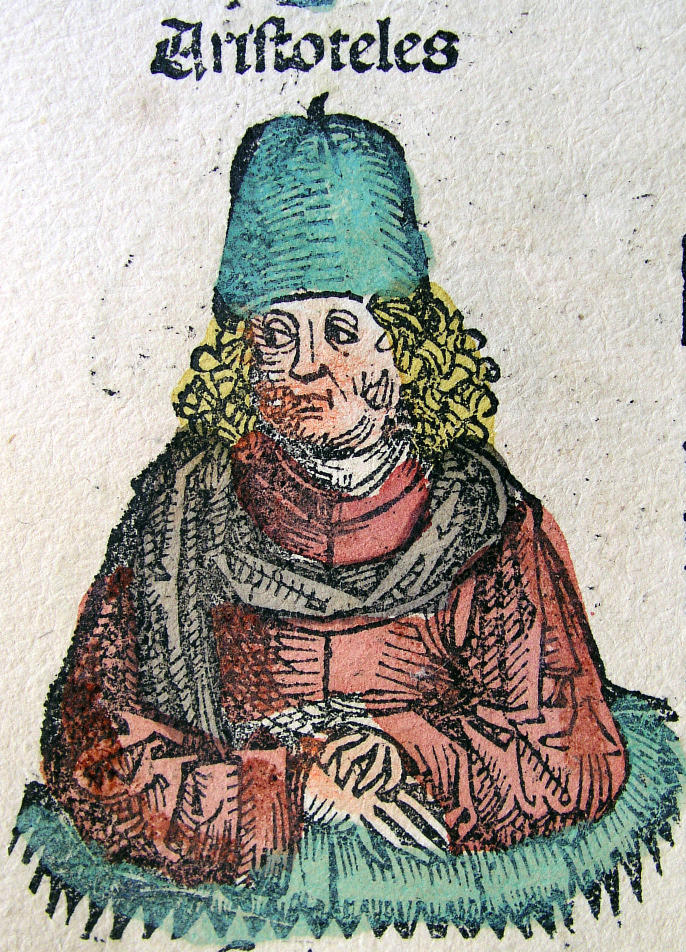
\includegraphics[width=0.3\textwidth]{Aristotle.jpg}
\end{center}
\caption{Аристотель глазами составителей Нюрнбергской хроники,
  1493}\label{fig:aristotle}
\end{figure}

Добавим лишь, что Аристотель в Нюрнбергской хронике
(см. Рис.~\ref{fig:aristotle}) был изображён в цвете, но в XXI веке
твёрдые копии сборников большинства конференций этим похвастаться не
могут. Поэтому в отношении всех цветных иллюстраций очень желательно
удостовериться в том, что и в чёрно-белом виде они не потеряют смысла.

При вставке графиков и диаграмм следует придерживаться тех же правил,
что и при вствке изображений. Отдельно настоятельно рекомендуется
графики и диаграммы врезать, используя векторные форматы изображений,
так как это, опять же, более предсказуемо выглядит в твёрдой копии.

Также следует убедиться, что использованное изображение не нарушает
ничьих авторских прав.

\subsection{Прочие врезки и ссылки (заголовок II уровня)}

Фрагменты текстов программ следует вставлять при помощи окружения
\texttt{lstlisting}:

\begin{lstlisting}[language=C,label=lst:code1]
int main()
{
    return 0;
}
\end{lstlisting}

Библиографические ссылки следует оформлять стандартными средствами
\texttt{\textbackslash{}cite} и
\texttt{\textbackslash{}bibitem}~\cite{medvedev2011}. BibTeX, BibLaTeX
и подобные средства хорошо работают в собственных руках на собственных
текстах, но, попав в чужие, делают сюрпризы.  Поэтому просьба либо их
не использовать, либо использовать так, чтобы организаторы конференции
об этом не знали.

\section{Заключение}

В документе были представлены основные стили текста и макросы, которые
могут быть использованы при форматировании тезисов конференции.
Собственные тезисы рекомендуется набирать в этом документе, заменяя
текст и заголовки на свои.

\begin{thebibliography}{8}

\bibitem{medvedev2011} Медведев О. Use case: отладка реализации RISC
  процессора для FPGA // % Материалы 2-й межвузовской научной
  конференции по проблемам информатики<<СПИСОК-2011>>. --- % 2011. ---
  С. 7--12.
  \href{http://math-science.math.spbu.ru/txt/math-science-2011.pdf}{http://math-science.math.spbu.ru/txt/math-science-2011.pdf}

\end{thebibliography}

\end{document}
